\documentclass[aspectratio=169, smaller]{beamer}
\setbeameroption{hide notes}
\mode<presentation>
\usepackage[]{slidespreamble}
\usepackage[]{math_commands}

% presentation title
\title{Meausure-theory view of probability}
\subtitle{handwavy and informal}

\begin{document}

\begin{frame}[t,plain]

%%%% Logos %%%%
\begin{textblock}{2}[0,0](0.5,0.5)
\includegraphics[width=1\textwidth]{id23_cairo-thws_logo_100pt_en_orange_NEU.png}
\end{textblock}

\begin{textblock}{10}[0,0](0,1.5)
\centering
{\Large Magda Gregorová}\\
\href{mailto:magda.gregorova@thws.de}{magda.gregorova@thws.de}

\vskip 2em
{\LARGE \color{thwspetrol} \inserttitle}\\
{\large \color{thwspetrol} \insertsubtitle}

\vskip 1em
\today

\vskip 2em
Licensed according to \href{https://creativecommons.org/licenses/by-sa/4.0}{CC-BY-SA 4.0}
\end{textblock}

\end{frame}



% \begin{frame}
% \layout
% \end{frame}

\begin{frame}[t]{Outline}
\setcounter{framenumber}{1}
\tableofcontents[]
\end{frame}

\section{Measures and probability}
\begin{frame}{Measures - assigning mass to sets}

\structure{Measurable space $(S, \salg)$}
\begin{itemize}
  \item $S$ - set (e.g., $\mR^d$, discrete set, etc.)
  \item $\salg$ - $\sigma$-algebra on $S$ (collection of measurable subsets of $S$)
  \begin{itemize}
    \item closed under complements and countable unions
    \item contains $\emptyset$ and $S$
  \end{itemize}
\end{itemize}

\vskip 1em
\structure{Measure $\mu$ on $(S, \salg)$ - function $\mu: \salg \to [0, \infty]$}
\begin{itemize}
  \item $\mu(\emptyset) = 0$
  \item countable additivity: for disjoint $\{A_i: i \in I\} \subseteq \salg$, $\mu\left( \bigcup_{i \in I} A_i \right) = \sum_{i \in I} \mu(A_i)$
\end{itemize}

\vskip 1em
\structure{Examples:}
\begin{itemize}
\item counting measure: $\#(A) = $ number of elements in $A$
\item Lebesgue measure on $\mR^d$: $\lambda(A) = $ volume of $A$
\end{itemize}

\end{frame}

\note[enumerate]
{
\item $\sigma$-algebra $\salg$ is collection of measurable sets (closed under complements and countable unions)
\item For practical purposes: think of $\salg$ as "all reasonable subsets"
\item Lebesgue measure generalizes notions of length, area, volume
\item Probability measure is just a finite measure normalized to total mass 1
\item This abstraction allows us to talk about probability rigorously, but we'll soon move to more practical objects
}

\begin{frame}{Probability measure}

\structure{Probability space $(S, \salg, \mP)$}
\begin{itemize}
  \item $S$ - sample space (possible outcomes of random experiment)
  \item $\salg$ - $\sigma$-algebra on $S$ (collection of events - sets of outcomes)
  \item $\mP: \salg \to [0, 1]$ - probability measure
  \begin{itemize}
    \item \alert{normalization: $\mP(S) = 1$}
    \item countable additivity (same as before)
  \end{itemize}
\end{itemize}

\vskip 1em
\structure{Interpretation:}
\begin{itemize}
\item random experiment produces outcome $s \in S$
\item event $A \in \salg$ is set of outcomes
\item $\mP(A)$ is probability that outcome lies in $A$
\end{itemize}

\vskip 1em
\structure{Abstract formalism:} $(S, \salg, \mP)$ gives rigorous framework\\
\alert{In practice: we work with random variables and their distributions}

\end{frame}

\note[enumerate]
{
\item Probability measure is just a normalized measure - total mass equals 1
\item The abstract probability space $(S, \salg, \mP)$ is often denoted $(\Omega, \mathscr{F}, \mP)$ in literature
\item Random experiment: think coin flip, dice roll, or any random process
\item Outcome $s \in S$: specific result of the experiment (e.g., "heads", or specific image)
\item Event $A \in \salg$: set of outcomes we're interested in (e.g., "at least 2 heads in 3 flips")
\item This level of abstraction separates the experiment from what we measure
\item But as we'll see next, we usually work with random variables that map outcomes to values we care about
}

\begin{frame}{Relationship: measures and probability}

\structure{Any finite measure can be normalized:}
\begin{itemize}
\item measure space $(S, \salg, \mu)$ with $\mu(S) < \infty$
\item define $\mP(A) = \frac{\mu(A)}{\mu(S)}$ for $A \in \salg$
\item then $(S, \salg, \mP)$ is probability space
\end{itemize}

\vskip 1em
\structure{Conversely: any probability measure can be scaled}
\begin{itemize}
\item probability space $(S, \salg, \mP)$
\item for any $c > 0$, $\mu = c \cdot \mP$ is finite measure with $\mu(S) = c$
\end{itemize}

\vskip 1em
\structure{Why this matters:}
\begin{itemize}
\item energy-based models: unnormalized measures $\mu(A) = \int_A e^{-E(s)} ds$
\item normalizing gives probability: $\mP(A) = \frac{1}{Z} \int_A e^{-E(s)} ds$ where $Z = \int_S e^{-E(s)} ds$
\item change of variables preserves this relationship
\end{itemize}

\end{frame}

\note[enumerate]
{
\item Normalization is just dividing by total mass
\item This shows probability measures are special cases of finite measures
\item Connection to statistical physics and energy-based models
\item Partition function $Z$ is the normalizing constant
\item When we transform measures, we transform probabilities - this is key for flows
}

\section{Random variables and distributions}
\begin{frame}{Random variable - moving to value space}

\structure{Random variable $X: S \to T$}
\begin{itemize}
  \item $(S, \salg, \mP)$ - probability space (random experiment)
  \item $(T, \mathscr{T})$ - measurable space (value space, e.g., $\mR^d$)
  \item $X$ - measurable function: $X^{-1}(B) \in \salg$ for all $B \in \mathscr{T}$
\end{itemize}

\vskip 1em
\structure{Interpretation:}
\begin{itemize}
\item random experiment produces outcome $s \in S$
\item we observe value $x = X(s) \in T$ - called \alert{realization} of $X$
\item $X$ maps abstract outcomes to concrete values we care about
\end{itemize}

\vskip 1em
\structure{Notation convention:}
\begin{itemize}
\item $X$ - random variable (the function itself)
\item $x$ - realization (a specific value in $T$)
\end{itemize}

\end{frame}

\note[enumerate]
{
\item Measurability is technical requirement - ensures we can measure probabilities after transformation
\item For continuous functions between nice spaces (e.g., $\mR^d$ with Borel sets), measurability is automatic
\item The value space $T$ is what we actually care about - numbers, vectors, images, etc.
\item Abstract sample space $S$ is often just formal device
\item In deep learning: we care about generated image $x$, not the random seed that produced it
\item Capital letter = random variable (random), lowercase = realization (fixed value)
}

\begin{frame}{Example: dice sum}

\structure{Roll two dice and sum them}

\vskip 0.5em
\structure{Setup:}
\begin{itemize}
\item sample space: $S = \{(1,1), (1,2), \ldots, (6,6)\}$ (36 outcomes)
\item probability: $\mP(\{(i,j)\}) = \frac{1}{36}$ for each outcome
\item random variable: $X(s_1, s_2) = s_1 + s_2$
\item value space: $T = \{2, 3, 4, \ldots, 12\}$
\end{itemize}

\vskip 1em
\structure{Realization:}
\begin{itemize}
\item if experiment gives $(3, 5) \in S$, then $x = X(3,5) = 8$
\item $x = 8$ is a realization of random variable $X$
\end{itemize}

\vskip 1em
\structure{Key point:}
\begin{itemize}
\item we care about the sum (value in $T$), not which dice showed what (outcome in $S$)
\item this motivates working with distribution on $T$ directly
\end{itemize}

\end{frame}

\note[enumerate]
{
\item Concrete example to ground the abstraction
\item Note: multiple outcomes in $S$ can give same value in $T$ (e.g., (2,6) and (3,5) both give sum 8)
\item This is why we need the distribution $P_X$ on $T$ - it aggregates probabilities
\item Example: $P_X(\{7\}) = \frac{6}{36}$ because 6 outcomes map to sum of 7
}

\begin{frame}{Distribution of random variable}

\structure{Given: $(S, \salg, \mP)$ and random variable $X: S \to T$}

\vskip 0.5em
\structure{Distribution (law) of $X$: probability measure $P_X$ on $(T, \mathscr{T})$}
\[
P_X(B) = \mP(X \in B) = \mP(\{s \in S: X(s) \in B\}), \quad B \in \mathscr{T}
\]

\vskip 1em
\structure{Interpretation:}
\begin{itemize}
\item $P_X(B)$ = probability that $X$ takes value in set $B$
\item $P_X$ lives on value space $T$, not on sample space $S$
\item $P_X$ is the push-forward of $\mP$ by $X$
\end{itemize}

\vskip 1em
\structure{Notation:} $X \sim P_X$ means "$X$ has distribution $P_X$"

\vskip 0.5em
\structure{Key point:} \alert{$P_X$ is a probability measure on $T$ - we can work with it directly!}

\end{frame}

\note[enumerate]
{
\item The distribution $P_X$ is completely determined by $X$ and $\mP$
\item Push-forward: probability "flows" from $S$ to $T$ through $X$
\item Once we have $P_X$, we can often forget about $(S, \salg, \mP)$
\item In practice: we specify $P_X$ directly without ever mentioning $S$
\item "X ~ N(0,1)" directly specifies distribution on $\mR$, no mention of underlying experiment
}

\begin{frame}{Working directly with distributions}

\structure{Two perspectives on probability:}

\vskip 1em
\structure{Formal perspective:}
\begin{itemize}
\item start with abstract probability space $(S, \salg, \mP)$
\item define random variable $X: S \to T$
\item derive distribution $P_X$ on value space $T$
\end{itemize}

\vskip 1em
\structure{Practical perspective (what we actually do):}
\begin{itemize}
\item \alert{directly specify distribution $P_X$ on value space $T$}
\item $(S, \salg, \mP)$ is implicit, often $S = T$ and $X = $ identity
\item notation: "$X \sim \mathcal{N}(0, I)$" directly defines Gaussian on $\mR^d$
\end{itemize}

\vskip 1em
\alert{From now on: we work with distributions on value spaces $T = \mR^d$}

\end{frame}

\note[enumerate]
{
\item This is the key conceptual shift for students
\item Abstract probability space is formal machinery, but not where we actually work
\item In generative modeling: we always work directly with distributions on $\mR^d$
\item The triplet $(\Omega, \mathscr{F}, \mP)$ is rarely mentioned in ML papers
\item Examples: "$z \sim p_{\text{prior}}$", "$x \sim p_{\text{data}}$" - these directly specify distributions
\item We're working with push-forward measures, but we specify them directly
\item Next section: we'll see different ways to represent these distributions (measure, CDF, density)
}


\section{Three ways to describe a distribution}
\begin{frame}{Three primary representations of a distribution}

\structure{Given random variable $X$ with values in $\mR^d$:}

\vskip 1em
\structure{1. Probability measure $P_X$}
\begin{itemize}
\item $P_X(A)$ - probability that $X \in A$
\item most fundamental
\end{itemize}

\vskip 0.5em
\structure{2. Cumulative distribution function (CDF) $F_X$}
\begin{itemize}
\item $F_X(x) = P_X((-\infty, x])$
\item always exists
\end{itemize}

\vskip 0.5em
\structure{3. Probability density function (PDF) $p_X$}
\begin{itemize}
\item $P_X(A) = \int_A p_X(x) \, dx$ when it exists
\item does not always exist
\end{itemize}

\vskip 1em
\alert{Three views of the same distribution}\\
{\small (other representations exist: characteristic function, MGF, etc.)}

\end{frame}

\note[enumerate]
{
\item This is a key conceptual point that students often miss
\item The measure, CDF, and density (when it exists) all describe the same distribution
\item Other representations exist: characteristic function $\phi_X(t) = E[e^{itX}]$, moment generating function $M_X(t) = E[e^{tX}]$, quantile function, etc.
\item We focus on these three because: (1) measure is fundamental, (2) CDF always exists, (3) density is what we compute with in ML
\item Measure is most general, CDF always exists, density only sometimes exists
\item In ML we mostly work with densities, but need to understand when they exist
\item Component-wise for CDF in $\mR^d$: $F_X(x_1, \ldots, x_d) = P_X((-\infty, x_1] \times \cdots \times (-\infty, x_d])$
}

\begin{frame}{Interlude: integration with respect to a measure}

\structure{Why we need this:} to connect measures with densities (functions)

\vskip 1em
\structure{Riemann integration (what you know):}
\[
\int_a^b f(x) \, dx = \text{area under curve}
\]

\vskip 1em
\structure{Generalization - integration w.r.t. measure $\mu$:}
\[
\int_A f \, d\mu
\]
\begin{itemize}
\item $A$ - any measurable set
\item $\mu$ - measure (weighs different parts of space)
\end{itemize}

\vskip 1em
\structure{Intuition:} weighted sum of $f$ over set $A$, weighted by measure $\mu$

\end{frame}

\note[enumerate]
{
\item Riemann integration: only over intervals, uses length/area/volume
\item Measure integration: over any measurable set, uses any measure
\item The measure $\mu$ determines how we "weigh" different parts of the space
\item This is a generalization that will let us work with probability measures
}

\begin{frame}{Interlude: Lebesgue measure and notation}

\structure{Lebesgue measure $\lambda$ on $\mR^d$}
\begin{itemize}
\item generalizes length/area/volume
\item $\lambda([a,b]) = b - a$ (length), $\lambda(A) = $ volume of $A$
\item integration: $\int_A f \, d\lambda = \int_A f(x) \, dx$ (familiar!)
\end{itemize}

\vskip 1em
\structure{Counting measure $\#$ on discrete/countable sets}
\begin{itemize}
\item $\#(A) = $ number of elements in $A$
\item integration: $\int_A f \, d\# = \sum_{x \in A} f(x)$ (discrete sum!)
\end{itemize}

\vskip 1em
\structure{Key insight:} \alert{integral notation unifies discrete and continuous}
\[
\int_A f \, d\mu \quad \begin{cases} 
= \int_A f(x) \, dx & \text{continuous (Lebesgue)} \\
= \sum_{x \in A} f(x) & \text{discrete (counting)}
\end{cases}
\]

\end{frame}

\note[enumerate]
{
\item Lebesgue measure is the "natural" measure on Euclidean space
\item For nice functions on nice sets: Riemann = Lebesgue integration
\item But Lebesgue integration works for much wider class of functions and sets
\item The notation $dx$ is shorthand for $d\lambda(x)$ (Lebesgue measure)
\item Counting measure: discrete sums become integrals!
\item Example with probability: $\int_{\mR^d} f \, dP_X = E[f(X)]$ works for both discrete and continuous X
\item This framework unifies discrete and continuous cases - no need for separate notation
}

\begin{frame}{Probability measure - the fundamental object}

\structure{Probability measure $P_X$ on $\mR^d$}
\begin{itemize}
\item assigns probability to measurable sets: $P_X(A) = \mP(X \in A)$
\item as integration: $P_X(A) = \int_A \, dP_X$
\end{itemize}

\vskip 1em
\structure{Key properties:}
\begin{itemize}
\item normalization: $P_X(\mR^d) = \int_{\mR^d} \, dP_X = 1$
\item for continuous distributions: $P_X(\{x_0\}) = \int_{\{x_0\}} \, dP_X = 0$ (single points have zero probability)
\end{itemize}

\vskip 1em
\structure{Properties:}
\begin{itemize}
\item most fundamental representation
\item works for discrete, continuous, and mixed distributions
\end{itemize}

\end{frame}

\note[enumerate]
{
\item We work with measurable sets - for practical purposes, "all reasonable subsets"
\item Single points have zero probability for continuous distributions because they have zero volume (Lebesgue measure)
\item Intuition: $P_X(\{x_0\}) = \int_{\{x_0\}} \, dP_X = 0$ because the set has zero measure
\item This is why we can't talk about "probability at a point" for continuous distributions - only density
\item Integration w.r.t. probability measure uses the framework from the interlude
\item The normalization property connects to what we saw in Section 1: any finite measure can be normalized
\item Measure is the fundamental object, but we often use CDF or density for computation
}

\begin{frame}{Cumulative distribution function (CDF)}

\structure{CDF $F_X: \mR^d \to [0, 1]$}

\vskip 0.5em
\structure{Definition (for $\mR$):}
\[
F_X(x) = P_X((-\infty, x]) = \mP(X \leq x)
\]

\vskip 1em
\structure{Example: Gaussian $X \sim \mathcal{N}(0, 1)$}
\[
F_X(x) = \int_{-\infty}^x \frac{1}{\sqrt{2\pi}} e^{-t^2/2} \, dt = \Phi(x)
\]
\begin{itemize}
\item $F_X(0) = 0.5$ (half the probability below 0)
\item $F_X(-\infty) = 0$, $F_X(\infty) = 1$
\end{itemize}

\vskip 1em
\structure{Properties:}
\begin{itemize}
\item always exists (for any distribution)
\item non-decreasing, right-continuous
\item $P_X((a, b]) = F_X(b) - F_X(a)$
\end{itemize}

\end{frame}

\note[enumerate]
{
\item CDF is unique representation - different distributions have different CDFs
\item For multidimensional case: $F_X(x_1, \ldots, x_d) = P_X((-\infty, x_1] \times \cdots \times (-\infty, x_d])$
\item CDF can have jumps (discrete distributions) or be continuous
\item Derivative of CDF gives density (when density exists)
\item In practice: we rarely work with CDF directly in ML, but it's theoretically important
}

\begin{frame}{Probability density function (PDF)}

\structure{PDF $p_X: \mR^d \to [0, \infty)$}

\vskip 0.5em
\structure{Definition:} when it exists,
\[
P_X(A) = \int_A p_X \, d\lambda = \int_A p_X(x) \, dx
\]
where $\lambda$ is Lebesgue measure (volume)

\vskip 0.5em
\structure{Interpretation:}
\begin{itemize}
\item $p_X$ is \alert{density} - probability per unit volume
\item $P_X$ is "weighted" by density: $dP_X = p_X \, d\lambda$ or $dP_X(x) = p_X(x) \, dx$
\item $p_X = \frac{dP_X}{d\lambda}$ - Radon-Nikodym derivative
\end{itemize}

\vskip 1em
\structure{Example: Gaussian $X \sim \mathcal{N}(0, 1)$}
\[
p_X(x) = \frac{1}{\sqrt{2\pi}} e^{-x^2/2}, \quad P_X([a,b]) = \int_a^b p_X(x) \, dx
\]
note: $p_X(0) \approx 0.40$ can be $> 1$ (it's density, not probability!)

\vskip 1em
\structure{When does density exist?} $P_X$ absolutely continuous w.r.t. $\lambda$

\end{frame}

\note[enumerate]
{
\item Density is what we actually compute and optimize in ML
\item Density is NOT probability - it's probability per unit volume
\item Common mistake: thinking $p(x)$ must be $\leq 1$. Not true!
\item Radon-Nikodym theorem guarantees density exists when absolutely continuous
\item Discrete distributions (point masses) do not have densities
\item Mixed distributions (part discrete, part continuous) do not have densities
}

\begin{frame}{Relationship between the three}

\structure{How they relate:}

\vskip 0.5em
\begin{center}
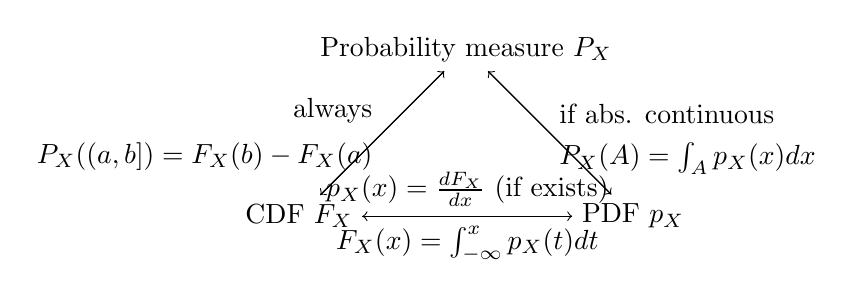
\begin{tikzpicture}[node distance=2cm]
\node (measure) {Probability measure $P_X$};
\node (cdf) [below left of=measure, node distance=3cm] {CDF $F_X$};
\node (pdf) [below right of=measure, node distance=3cm] {PDF $p_X$};

\draw[->] (measure) -- (cdf) node[midway,above left] {always};
\draw[->] (measure) -- (pdf) node[midway,above right] {if abs. continuous};
\draw[->] (pdf) -- (cdf) node[midway,below] {$F_X(x) = \int_{-\infty}^x p_X(t) dt$};
\draw[->] (cdf) -- (pdf) node[midway,above] {$p_X(x) = \frac{dF_X}{dx}$ (if exists)};
\draw[->] (pdf) -- (measure) node[midway,below right] {$P_X(A) = \int_A p_X(x) dx$};
\draw[->] (cdf) -- (measure) node[midway,below left] {$P_X((a,b]) = F_X(b) - F_X(a)$};
\end{tikzpicture}
\end{center}

\vskip 1em
\structure{Key points:}
\begin{itemize}
\item measure $\to$ CDF: always possible
\item measure $\to$ PDF: only when absolutely continuous
\item in ML: we almost always work with PDFs (assume absolute continuity)
\end{itemize}

\end{frame}

\note[enumerate]
{
\item This diagram shows all the relationships
\item Most fundamental: measure
\item Most general representation that always exists: CDF
\item Most convenient for computation: PDF (when it exists)
\item In deep learning: we assume our distributions have densities
\item This is reasonable for continuous distributions on $\mR^d$
}

\begin{frame}{Examples: discrete, continuous, mixed}

\structure{Discrete: $X \in \{0, 1, 2\}$ with $P_X(\{k\}) = 1/3$}
\begin{itemize}
\item measure: $P_X(\{0\}) = P_X(\{1\}) = P_X(\{2\}) = 1/3$
\item CDF: $F_X(x) = \begin{cases} 0 & x < 0 \\ 1/3 & 0 \leq x < 1 \\ 2/3 & 1 \leq x < 2 \\ 1 & x \geq 2 \end{cases}$ (step function)
\item PDF: \alert{does not exist} (point masses)
\end{itemize}

\vskip 1em
\structure{Continuous: $X \sim \mathcal{N}(0, 1)$}
\begin{itemize}
\item measure: $P_X(A) = \int_A \frac{1}{\sqrt{2\pi}} e^{-x^2/2} dx$
\item CDF: $F_X(x) = \Phi(x)$ (smooth, no jumps)
\item PDF: $p_X(x) = \frac{1}{\sqrt{2\pi}} e^{-x^2/2}$ \alert{exists}
\end{itemize}

\vskip 0.5em
\structure{Mixed: half point mass at 0, half uniform on $[0,1]$}
\begin{itemize}
\item PDF: \alert{does not exist} (has point mass at 0)
\end{itemize}

\end{frame}

\note[enumerate]
{
\item These examples show when density exists and when it doesn't
\item Discrete: CDF has jumps, no density
\item Continuous: CDF is smooth, density exists
\item Mixed: combination, no density
\item In generative modeling: we work with continuous distributions, so densities exist
\item Point masses and discrete distributions don't have densities w.r.t. Lebesgue measure
}


\section{Transformations and push-forward}
\begin{frame}{Transformations of random variables}

\structure{Setup:} 
\begin{itemize}
\item $X$ - random variable with values in $T$ (e.g., $\mR^d$)
\item $P_X$ - distribution of $X$ on $T$
\item $g: T \to U$ - measurable function (transformation)
\item $Y = g(X)$ - transformed random variable with values in $U$
\end{itemize}

\vskip 1em
\structure{Question:} If we know $P_X$, what is the distribution $P_Y$ of $Y = g(X)$?

\vskip 1em
\structure{Examples in ML:}
\begin{itemize}
\item $X \sim \mathcal{N}(0, I)$ (simple), $g$ is neural network, $Y = g(X)$ (complex model distribution)
\item data transformation: $X$ is data, $g$ encodes to latent space
\end{itemize}

\end{frame}

\note[enumerate]
{
\item This is the fundamental question in generative modeling
\item We transform a simple distribution to get a complex one
\item The transformation $g$ is typically a neural network
\item We work directly with distributions on value spaces (as established in Section 2)
\item No need to refer back to abstract probability space $(S, \salg, \mP)$
}


\begin{frame}{Push-forward measure}

\structure{Answer:} distribution of $Y = g(X)$ is the push-forward of $P_X$ by $g$

\vskip 0.5em
\structure{Definition:} $P_Y$ on $U$ defined by
\[
P_Y(C) = P_X(g^{-1}(C)) \quad \text{for } C \subseteq U
\]
where $g^{-1}(C) = \{x \in T: g(x) \in C\}$ is the pre-image

\vskip 1em
\centering
\scalebox{0.55}{
\begin{tikzpicture}[>=Stealth]
% LEFT: domain T with mesh and rectangular g^{-1}(C)
\begin{scope}[shift={(-5,0)}]
    \node at (0,2) {$T$};
    % Mesh (vertical)
    \foreach \x in {-1.5,-1,...,1}
        \draw[gray!70] (\x,-2) -- (\x,2);
    % Mesh (horizontal)
    \foreach \y in {-1.5,-1,...,1.5}
        \draw[gray!70] (-2,\y) -- (1.5,\y);
    % Preimage region g^{-1}(C): ALIGNED WITH GRID
    \fill[blue!25,opacity=0.5] (-1,-1) rectangle (0,1);
    \draw[blue!60,thick] (-1,-1) rectangle (0,1);
    \node[blue!80] at (-0.5,0) {$g^{-1}(C)$};
\end{scope}
% Middle arrow: g
\draw[->,thick] (-2.5,0.5) -- (-0.5,0.5) node[midway,above] {$g: T \to U$};
\draw[<-,thick] (-2.5,-0.5) -- (-0.5,-0.5) node[midway,above] {preimage};
\node at (-1.5,1.8) {\color{carnelian}$P_X(g^{-1}(C)) = P_Y(C)$};
% RIGHT: codomain U with warped mesh + image C
\begin{scope}[shift={(2,0)}]
    \node at (0,2) {$U$};
    % Warped vertical mesh lines
    \foreach \x in {-1.5,-1,...,1}
    \draw[gray!70,domain=-2:2,smooth,variable=\t]
        plot ({0.9*\x + 0.5*sin(\t r)}, {\t + 0.5*sin(\x r)});
    % Warped horizontal mesh lines
    \foreach \y in {-1.5,-1,...,1.5}
    \draw[gray!70,domain=-2:1.5,smooth,variable=\t]
        plot ({0.9*\t + 0.5*sin(\y r)}, {\y + 0.5*sin(\t r)});
    % Image region C
    \begin{scope}
        \fill[blue!25,opacity=0.5]
            plot[domain=-1:0,smooth,variable=\x]
                ({0.9*\x + 0.5*sin(-1 r)}, {-1 + 0.5*sin(\x r)})
            -- plot[domain=-1:1,smooth,variable=\y]
                ({0.9*0 + 0.5*sin(\y r)}, {\y + 0.5*sin(0 r)})
            -- plot[domain=0:-1,smooth,variable=\x]
                ({0.9*\x + 0.5*sin(1 r)}, {1 + 0.5*sin(\x r)})
            -- plot[domain=1:-1,smooth,variable=\y]
                ({0.9*(-1) + 0.5*sin(\y r)}, {\y + 0.5*sin(-1 r)})
            -- cycle;
        \draw[blue!60,thick]
            plot[domain=-1:0,smooth,variable=\x]
                ({0.9*\x + 0.5*sin(-1 r)}, {-1 + 0.5*sin(\x r)})
            -- plot[domain=-1:1,smooth,variable=\y]
                ({0.9*0 + 0.5*sin(\y r)}, {\y + 0.5*sin(0 r)})
            -- plot[domain=0:-1,smooth,variable=\x]
                ({0.9*\x + 0.5*sin(1 r)}, {1 + 0.5*sin(\x r)})
            -- plot[domain=1:-1,smooth,variable=\y]
                ({0.9*(-1) + 0.5*sin(\y r)}, {\y + 0.5*sin(-1 r)})
            -- cycle;
        \node[blue!80] at (-0.4,-0.1) {$C$};
    \end{scope}
\end{scope}
\end{tikzpicture}
}

\vskip 0.5em
\structure{Intuition:} probability of $Y$ landing in $C$ equals probability of $X$ being in pre-image

\end{frame}

\note[enumerate]
{
\item Push-forward is how distributions transform under functions
\item The pre-image $g^{-1}(C)$ is the set of points in $T$ that map to $C$
\item Diagram shows: regular grid in $T$ becomes warped in $U$, but probability is preserved
\item This is well-defined because $g$ is measurable
\item In ML: $g$ is neural network, $P_X$ is simple distribution (e.g., Gaussian), $P_Y$ is complex model distribution
\item We're working directly with distributions $P_X$ and $P_Y$, not going back to abstract probability space
}

\begin{frame}{Example: uniform distribution and affine transformation}

\structure{Setup:} $X \sim \text{Uniform}[0, 1]$, transformation $g(x) = 2x + 3$, find distribution of $Y = g(X)$

\vskip 0.5em
\begin{center}  
\scalebox{0.75}{
\begin{tikzpicture}[>=Stealth]
% LEFT: X ~ Uniform[0,1]
\begin{scope}[shift={(-4,0)}]
    \node at (1.8,3) {$X \sim \text{Uniform}[0,1]$};
    
    % Axis
    \draw[->] (-0.5,0) -- (4,0) node[right] {$x$};
    \draw[->] (0,-0.3) -- (0,2.5) node[above] {$p_X(x)$};
    
    % Uniform density
    \fill[blue!20,opacity=0.6] (0,0) rectangle (3,2);
    \draw[blue,thick] (0,0) -- (0,2) -- (3,2) -- (3,0);
    
    % Highlighted interval [0.25, 0.75] (50% probability)
    \fill[blue!50,opacity=0.8] (0.75,0) rectangle (2.25,2);
    
    % Labels
    \node[below] at (0,0) {$0$};
    \node[below] at (3,0) {$1$};
    \node[left] at (0,2) {$1$};
    \node[below] at (0.75,0) {\small $0.25$};
    \node[below] at (2.25,0) {\small $0.75$};
   
    % Probability in middle
    \node at (1.5,1) {$P_X(g^{-1}(C)) = 0.5$};
    
    % Probability annotation
    \draw[<->,thick] (0.75,-0.8) -- (2.25,-0.8);
    \node[below] at (1.5,-0.8) {\small length $= 0.5$};
    \node[above] at (1.5,-0.8) {\small $g^{-1}(C)$};
\end{scope}

% Arrow with transformation
\node at (1.5,-0.8) {\color{carnelian}$P_X(g^{-1}(C)) = P_Y(C) = 0.5$};
\draw[->,very thick] (-0,1.5) -- (2.5,1.5) node[midway,above] {$g(x) = 2x+3$};
\draw[<-,thick] (-0,0.5) -- (2.5,0.5) node[midway,above] {preimage};

% RIGHT: Y ~ Uniform[3,5]
\begin{scope}[shift={(0.5,0)}]
    \node at (5.5,3) {$Y \sim \text{Uniform}[3,5]$};
    
    % Axis
    \draw[->] (2.5,0) -- (9.5,0) node[right] {$y$};
    \draw[->] (3,-0.3) -- (3,2.5) node[above] {$p_Y(y)$};
    
    % Uniform density on [3,5]
    \fill[red!20,opacity=0.6] (3,0) rectangle (9,1);
    \draw[red,thick] (3,0) -- (3,1) -- (9,1) -- (9,0);
    
    % Highlighted interval [3.5, 4.5] = g([0.25, 0.75])
    \fill[red!50,opacity=0.8] (4.5,0) rectangle (7.5,1);
    
    % Labels
    \node[below] at (3,0) {$3$};
    \node[below] at (9,0) {$5$};
    \node[left] at (3,1) {$\frac{1}{2}$};
    \node[below] at (4.5,0) {\small $3.5$};
    \node[below] at (7.5,0) {\small $4.5$};
      
    % Probability in middle
    \node at (6,0.5) {$P_Y(C) = 0.5$};
    
    % Probability annotation
    \draw[<->,thick] (4.5,-0.8) -- (7.5,-0.8);
    \node[below] at (6,-0.8) {\small length $= 1$};
    \node[above] at (6,-0.8) {\small $C$};
\end{scope}
\end{tikzpicture}
}
\end{center}

\vskip 0.5em
\structure{Key insight:}
\begin{itemize}
\item transformation $g$ stretches the space: interval $[0.25, 0.75]$ becomes $[3.5, 4.5]$ (length doubles)
\item same probability (0.5) must be distributed over larger space
\item $\Rightarrow$ density decreases: $p_Y = \frac{1}{2} p_X$
\end{itemize}

\alert{Stretching space $\Rightarrow$ density decreases (probability conserved)}

\end{frame}

\note[enumerate]
{
\item This is a simple concrete example showing push-forward
\item The preimage calculation: solve $a \leq 2x+3 \leq b$ for $x$
\item Uniform on $[0,1]$: $P_X([a,b]) = b - a$ when $[a,b] \subseteq [0,1]$
\item After transformation: still uniform, but on $[3,5]$ instead of $[0,1]$
\item The scaling factor 2 will become important when we look at densities (Jacobian)
\item This example shows: push-forward preserves the "shape" but changes location and scale
}

\section{Change of variables at density level}
\begin{frame}{From push-forward to change of variables}

\structure{What we saw:} uniform distribution + affine transformation
\begin{itemize}
\item $X \sim \text{Uniform}[0,1]$, $g(x) = 2x + 3$, $Y = g(X)$
\item stretching by factor 2 $\Rightarrow$ density halves
\item easy to compute: $p_Y = \frac{1}{2}$
\end{itemize}

\vskip 1em
\structure{General question:}\\
Given arbitrary distribution $p_X$ and transformation $g$, how do we compute $p_Y$?

\vskip 1em
\structure{Challenge:}
\begin{itemize}
\item not just uniform distributions
\item not just affine transformations
\item need general formula relating $p_Y$ to $p_X$ and $g$
\end{itemize}

\vskip 0.5em
\alert{Goal: derive the change of variables formula with Jacobian determinant}

\end{frame}

\note[enumerate]
{
\item The uniform example was special - constant density, linear transformation
\item In ML: we use complex distributions (Gaussian, data distributions) and complex transformations (neural networks)
\item Need to understand how densities transform in general
\item This is the change of variables formula - fundamental for normalizing flows, diffusion models, etc.
}

\begin{frame}{Step 1: Start from push-forward}

\structure{Recall:} push-forward at measure level
\[
P_Y(C) = P_X(g^{-1}(C))
\]

\vskip 1em
\structure{Express using densities:} (assuming densities exist)
\[
P_Y(C) = \int_C p_Y(y) \, dy = \int_{g^{-1}(C)} p_X(x) \, dx = P_X(g^{-1}(C))
\]

\vskip 1em
\structure{Key observation:}
\begin{itemize}
\item left side: integrate $p_Y$ over $C$ in $y$-space
\item right side: integrate $p_X$ over $g^{-1}(C)$ in $x$-space
\item same probability, different spaces
\end{itemize}

\vskip 0.5em
\structure{Idea:} change variables in right side from $x$ to $y = g(x)$

\end{frame}

\note[enumerate]
{
\item This is the starting point - push-forward expressed with densities
\item Left side: probability in target space $U$ (using $p_Y$)
\item Right side: probability in source space $T$ (using $p_X$)
\item They're equal by push-forward definition
\item Next: use change of variables from calculus to transform the right integral
}

\begin{frame}{Step 2: Change of variables in integrals}

\structure{From calculus:} change of variables formula
\[
\int_{g^{-1}(C)} f(x) \, dx = \int_C f(g^{-1}(y)) \left| \det \frac{\partial g^{-1}}{\partial y}(y) \right| \, dy
\]

\vskip 0.5em
Assuming $g: \mR^d \to \mR^d$ is invertible and differentiable

\vskip 1em
\structure{The Jacobian determinant:}
\begin{itemize}
\item $\frac{\partial g^{-1}}{\partial y}$ is the $d \times d$ Jacobian matrix of $g^{-1}$
\item $\det \frac{\partial g^{-1}}{\partial y}$ measures local volume change
\item absolute value: $\left| \det \frac{\partial g^{-1}}{\partial y} \right|$
\end{itemize}

\vskip 1em
\structure{Intuition:} $dx = \left| \det \frac{\partial g^{-1}}{\partial y} \right| dy$ (infinitesimal volume scaling)

\end{frame}

\note[enumerate]
{
\item This is the standard change of variables from multivariable calculus
\item The Jacobian matrix contains all partial derivatives
\item Its determinant tells us how volumes scale under the transformation
\item We need absolute value because we're integrating (measure must be positive)
\item For $d=1$: this reduces to $|dx/dy|$ or $|1/g'(x)|$
\item We can also write in terms of $g$ instead of $g^{-1}$ (next slide)
}

\begin{frame}{Step 3: Apply to our setting}

\structure{Apply change of variables:}
\[
\int_{g^{-1}(C)} p_X(x) \, dx = \int_C p_X(g^{-1}(y)) \left| \det \frac{\partial g^{-1}}{\partial y}(y) \right| \, dy
\]

\vskip 1em
\structure{But we also have:}
\[
\int_{g^{-1}(C)} p_X(x) \, dx = \int_C p_Y(y) \, dy
\]
by push-forward

\vskip 1em
\structure{Therefore:}
\[
\int_C p_Y(y) \, dy = \int_C p_X(g^{-1}(y)) \left| \det \frac{\partial g^{-1}}{\partial y}(y) \right| \, dy
\]

\vskip 0.5em
Since this holds for all $C$, the integrands must be equal!

\end{frame}

\note[enumerate]
{
\item This is the key step: combining push-forward with change of variables
\item We have two expressions for the same integral
\item Both integrate over $C$ in $y$-space
\item The integrands must be equal
\item This gives us the formula for $p_Y$ in terms of $p_X$
}

\begin{frame}{Step 4: Change of variables formula}

\structure{Result:}
\[
p_Y(y) = p_X(g^{-1}(y)) \left| \det \frac{\partial g^{-1}}{\partial y}(y) \right|
\]

\vskip 1em
\structure{Alternative form:} using inverse function theorem
\[
\det \frac{\partial g^{-1}}{\partial y}(y) = \frac{1}{\det \frac{\partial g}{\partial x}(g^{-1}(y))}
\]

Therefore:
\[
p_Y(y) = p_X(g^{-1}(y)) \left| \det \frac{\partial g}{\partial x}(g^{-1}(y)) \right|^{-1}
\]

\vskip 1em
\structure{Common notation:} $J_g(x) = \frac{\partial g}{\partial x}(x)$ (Jacobian of $g$)
\[
\boxed{p_Y(y) = \frac{p_X(g^{-1}(y))}{|\det J_g(g^{-1}(y))|}}
\]

\end{frame}

\note[enumerate]
{
\item This is the change of variables formula!
\item First form: uses Jacobian of $g^{-1}$ (inverse transformation)
\item Second form: uses Jacobian of $g$ (forward transformation) - usually more convenient
\item Inverse function theorem: $J_{g^{-1}}(y) = [J_g(g^{-1}(y))]^{-1}$
\item Determinants: $\det(A^{-1}) = 1/\det(A)$
\item The Jacobian determinant in denominator - this is key for normalizing flows
}

\begin{frame}{Geometric interpretation of Jacobian}

\structure{What does $|\det J_g(x)|$ mean geometrically?}

\vskip 0.5em
Local volume scaling factor at point $x$

\vskip 1em
\structure{In 1D:} $g: \mR \to \mR$
\[
|\det J_g(x)| = |g'(x)| = \text{local stretching factor}
\]

\vskip 1em
\structure{Example:} $g(x) = 2x + 3$
\begin{itemize}
\item $g'(x) = 2$ everywhere
\item stretches by factor 2 everywhere
\item density: $p_Y(y) = \frac{p_X(g^{-1}(y))}{2}$ (matches our uniform example!)
\end{itemize}

\vskip 1em
\structure{In higher dimensions:}
\begin{itemize}
\item $|\det J_g(x)|$ measures how $g$ stretches/compresses volume near $x$
\item $|\det J_g(x)| > 1$: expansion $\Rightarrow$ density decreases
\item $|\det J_g(x)| < 1$: contraction $\Rightarrow$ density increases
\end{itemize}

\end{frame}

\note[enumerate]
{
\item The Jacobian determinant has clear geometric meaning
\item It tells us how volumes change under the transformation
\item In 1D: just the derivative (slope)
\item Our uniform example: constant Jacobian = 2, density halves
\item In general: Jacobian varies with position $x$
\item This is why neural networks can create complex distributions - varying Jacobian
\item Key principle: stretching space → lower density, compressing space → higher density
}

\end{document}